\documentclass{article}
\usepackage{graphicx}
\usepackage{amsmath}
\usepackage{mathtools}
\usepackage[margin=1in]{geometry}
\author{Graham Roberts}
\title{Research update June 17 2016}
\begin{document}
\maketitle
\section{introduction}

This is the first blog post of the summer work period.  This is also the first blog post since Scholars' Week.  As such this will serve as a good marker of exactly where we stand, relative to the road map, and where I think we should go next.  First off, I have made very little progress since Scholars' Week.  In the month since then, I have sunk around 20-30 hours into the project, and seem to be finding the same thing we have been for months;  We cannot properly identify the same members that other surveys did, and we cannot reliably eliminate all contaminants when our probability is based off of position and proper motion.  I think discontinuing to consider position might be helpful in our project.  I have looked at the data from Sheikhi et. al. and that looks promising.

\section{where we stand vs Deacon \& Hambly}

First thing first we decided to look at how our results compare to those of Deacon \& Hambly.  In short the correlation between the two is minimal at best.  Matching stars that they computed to be high probability members to their probability as compute by me revealed that the corelation between the two is borderline nonexistent.  I created plots of the two probabilites plotted with respect to each other. 

\begin{center}
\includegraphics[width=.4\textwidth]{/home/groberts/p_memVDHp_mem} 
\includegraphics[width=.4\textwidth]{/home/groberts/p_memVp_memDHs}
\end{center}

While neither of those realy shows much correlation between our selection methods I did include the plot where I only look at my selection method based off of Proper motion, althought that is still normalized by the attempt to find 700 members in the cluster through both proper motion and position.  I wiil look more at the decision to strongly consider proper motion, while largely disregarding position other than as an initial selection later in the blog post.  I then decided to analyze how Deacon and Hambly's membership probabilities relate to the position and proper motion of he stars.  This revealed slighly more meaningful information.

\begin{center}
\includegraphics[width=.4\textwidth]{/home/groberts/HDp_memVdegsep}
\includegraphics[width=.4\textwidth]{/home/groberts/DHp_memVmasyrsep}
\end{center}

This demonstrates the clear trend for high probabilty members to be close to the mean values of proper motion of the cluster, which is what what we would expect.  It also shows that while there are few members far away from the central position of the cluster their distribution  id fairly large.  The key problem is that Deacon \& Hambly did not calculate membership probabiity as a clear function of proper motion. The probability values while all high span the entire range of probabilities even at very small proper motions.  The only data provided was on stars calculated to have greater than about .6 probability of being a member. There is no reason to believe that stars with lower probability than that also had similar proper motion. I expect they were few in number, especially considering plots of proper motion space, there are only a small number of stars at the mean proper moion of the cluster.  The key thing they did differently than me was also basing membership probabilities off of photometric properties, which we have decided against doing until we can estimate an age estimate for the cluster. 

\section{Sheikhi data}

I also looked at the data provided by the Sheikhi study.  The Sheikhi survey has a list of 810 or so members, of which 410 match within 3 arcseconds to stars in the catalog from which I was working, and 157 match to previously known members.  The membership table provided list 53 stars that are supposed members of the Deacon \& Hambly table.  That said I created a CMD for the stars in the sheikhi catalog with the J and Ks magnitudes included in the table.  There are domr stars near the turn off which is encouraging.  I also created plots of proper motion in right acension and proper motion in declination of the members selected by Sheikhi.

\begin{center}
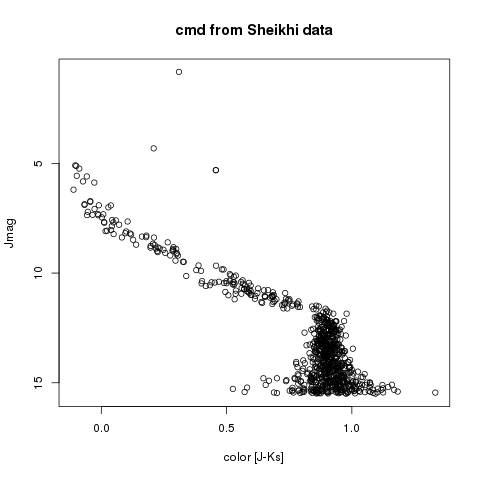
\includegraphics[width=.4\textwidth]{isochroneofsheikhidata}
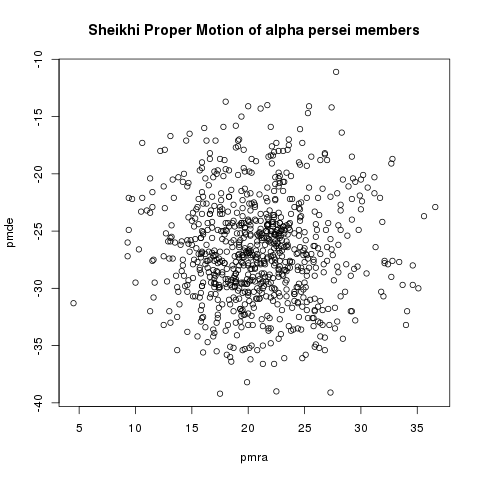
\includegraphics[width=.4\textwidth]{sheikhiProperMotions.png}
\end{center}

\section{Probability based off of position questions}

So up until this point in this blog entry I have expressed concern with assigning probabilities of membership based off of position.  It seems that position is useful in determinig which stars are worth looking at to begin with, but little more than that.  Neither mine nor Deacon \& Hambly's selection showed much correlation to position.  Forthis reason I may compute membership probabilities without computing radial distance in position in the future. That said I still have yet to incorporate the parallax distance of position from the recent URAT1 release.  Limiting position in three dimensions should provide very valuable information membership probability.  

\section{Next Steps}

Before next week I intend to have viewed the URAT1 parallax data, hopefully found a few new bright stars, hopefully near the turn off. I will compile a list of the all the stars in the surveys of Prosser, Deacon \& Hambly, and Sheikhi.  I will add selections I make incorporating parralax, and I will generate a color magnitude diagram.  If I have time I will begin fitting the PARSEC models, although you expressed concern with their uncertainty.  In the less immediate, but not too distant future I will finish fitting the PARSEC models and analyze uncertainty with my fit.  I will use the model I have fit to A determine age, and B discover new members for the APOGEE project, because all the work I have seen uses both proper motion and photometric data to compute membership.
\end{document}

